\problemname{\#include "main.hpp"}
%% plainproblemname: #include "main.hpp"

\noindent
Louise har tillbringat det senaste året med att förbereda sig för en kommande programmeringstävling. 
Intressant nog tillåter denna tävling endast deltagare att använda ett forntida programspråk kallat \verb|H++|.

I \verb|H++|, som är ett objektorienterat språk, kan man inkludera externa filer i sitt program under kompileringen
genom att skriva raden:

\begin{verbatim}
#include "file.hpp"
\end{verbatim}

När kompilatorn stöter på denna rad inkluderar den innehållet från den angivna filen (\texttt{file.hpp}) i den
aktuella filen på platsen där \verb|#include|-direktivet finns. Innehållet i \texttt{file.hpp} kopieras och
klistras in där \verb|#include|-kommandot finns, vilket ersätter den raden i filen.

En viktig egenskap hos \verb|H++| är att filer kan inkludera sig själva. Det innebär att om en fil som heter
\texttt{main.hpp} innehåller en rad som:

\begin{verbatim}
#include "main.hpp"
\end{verbatim}

innebär det att filen \texttt{main.hpp} kommer inkluderas rekursivt, där innehållet i \texttt{main.hpp} kopieras
och klistras in igen. Detta skapar en självreplikerande cykel som kan upprepas flera gånger, vilket potentiellt
resulterar i en väldigt stor fil. För att förhindra detta från att bli en oändlig loop introducerade skaparen av
\verb|H++| en rekursionsgräns, som låter användaren sätta ett maximalt antal rekursiva inkluderingar
(betecknat som $k$).

Detta innebär att om filen befinner sig på den $k$-te rekursionsnivån, 
kommer den endast att inkludera raden \verb|#include "main.hpp"| på den specifika nivån av filen. 
Efter $k$ lager av inkluderingar stoppas rekursionen.

När filen kompileras tilldelas varje rad i den resulterande filen ett unikt radnummer,
där första raden har radnummer 1.

Men när Louise försöker använda denna funktion stöter hon på många kompileringsfel. 
Specifikt får hon $Q$ kompileringsfel, var och en anger ett radnummer i den slutliga kompilerade filen där ett
fel inträffade. Dessa radnummer motsvarar den kompilerade filen, där innehållet från \texttt{main.hpp} har kopierats
flera gånger på grund av de rekursiva inkluderingarna.

Problemet är att dessa radnummer är baserade på den kompilerade versionen av filen, inte den ursprungliga filen. 
Som ett resultat behöver Louise hjälp att ta reda på vilka felraderna i den kompilerade filen faktiskt motsvarar i
den ursprungliga koden.

\section*{Indata}
\noindent
Den första raden innehåller tre heltal $N$, $k$ och $Q$
($1 \leq N \leq 10^6$, $1 \leq k \leq 10^9$, $1 \leq Q \leq 10^5$),
$N$ är antalet rader i den ursprungliga filen \texttt{main.hpp}, 
$k$ är rekursionsgränsen (det maximala antalet rekursiva inkluderingar), och $Q$ är antalet kompileringsfel.

De följande $N$ raderna innehåller varje en rad kod från \texttt{main.hpp}. Var och en av dessa rader består av högst
35 utskrivbara ASCII-tecken. \texttt{main.hpp} kommer inte att inkludera andra filer än \texttt{main.hpp}.

De följande $Q$ raderna innehåller var och en ett heltal $p_i$ ($1 \leq p_i \leq 10^{12}$), vilket indikerar ett
radnummer i den kompilerade filen där ett fel uppstod. Det är garanterat att $p_i$ kommer att vara ett giltigt
radnummer i den kompilerade filen.

\textbf{OBS: } Värdet på $p_i$ kommer inte att få plats i ett 32-bitars heltal, så var medveten om att det kan
överflöda om du använder C++. Notera också att det finns en stor mängd indata och utdata, så det rekommenderas
att använda snabb in-/utdata (IO).

\section*{Utdata}
\noindent
För varje av de $Q$ felen, skriv ut motsvarande kodrad från den ursprungliga filen \texttt{main.hpp}
som motsvarar radnumret i den kompilerade filen. 
Utdata ska ges i samma ordning som de $Q$ felraderna anges.

\section*{Poängsättning}
Din lösning kommer att testas på en mängd testfallsgrupper.
För att få poäng för en grupp så måste du klara alla testfall i gruppen.

\noindent
\begin{tabular}{| l | l | p{12cm} |}
  \hline
  \textbf{Grupp} & \textbf{Poäng} & \textbf{Gränser} \\ \hline
  $1$    & $2$        & Raden \verb|#include "main.hpp"| förekommer exakt en gång. \\ \hline
  $2$    & $3$        & $k = 1$ \\ \hline
  $3$    & $9$        & $N = 2$ \\ \hline
  $4$    & $12$       & $N,Q \leq 100$ och $k \leq 10$. \\ \hline 
  $5$    & $13$       & $N \leq 10^3, Q \leq 10^4$ och $k \leq 100$. \\ \hline 
  $6$    & $11$       & $Q \leq 10^4$ och $k \leq 500$. \\ \hline 
  $7$    & $18$       & $k \leq 10^3$ \\ \hline 
  $8$    & $23$       & $k \leq 5\cdot10^5$ \\ \hline 
  $9$    & $9$        & Inga ytterligare begränsningar. \\ \hline
\end{tabular}

\section*{Förklaring av exempelfall}
Det första exemplet har endast 1 rad med \verb|#include "main.hpp"|. 
Rad 1, 3 och 5 i den kompilerade filen motsvarar rad 1, 3 och 5 i den ursprungliga filen. 
Rad 8 i den kompilerade filen motsvarar rad 4 i den ursprungliga filen.
Rad 13 i den kompilerade filen motsvarar rad 5 i den ursprungliga filen.

\begin{figure}[h]
  \centering
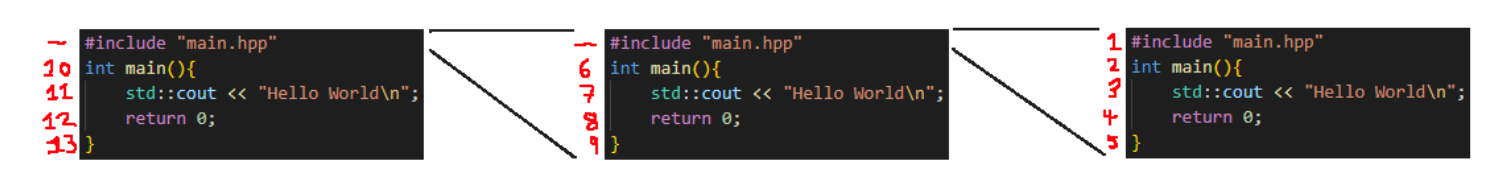
\includegraphics[width=\textwidth]{include1.png}
  \caption{Illustration av exempel 1 med ursprungligen 5 rader. De röda siffrorna visar motsvarande radnummer
  i den kompilerade filen.}
  \label{fig:include1}
\end{figure}

\begin{figure}[h]
  \centering
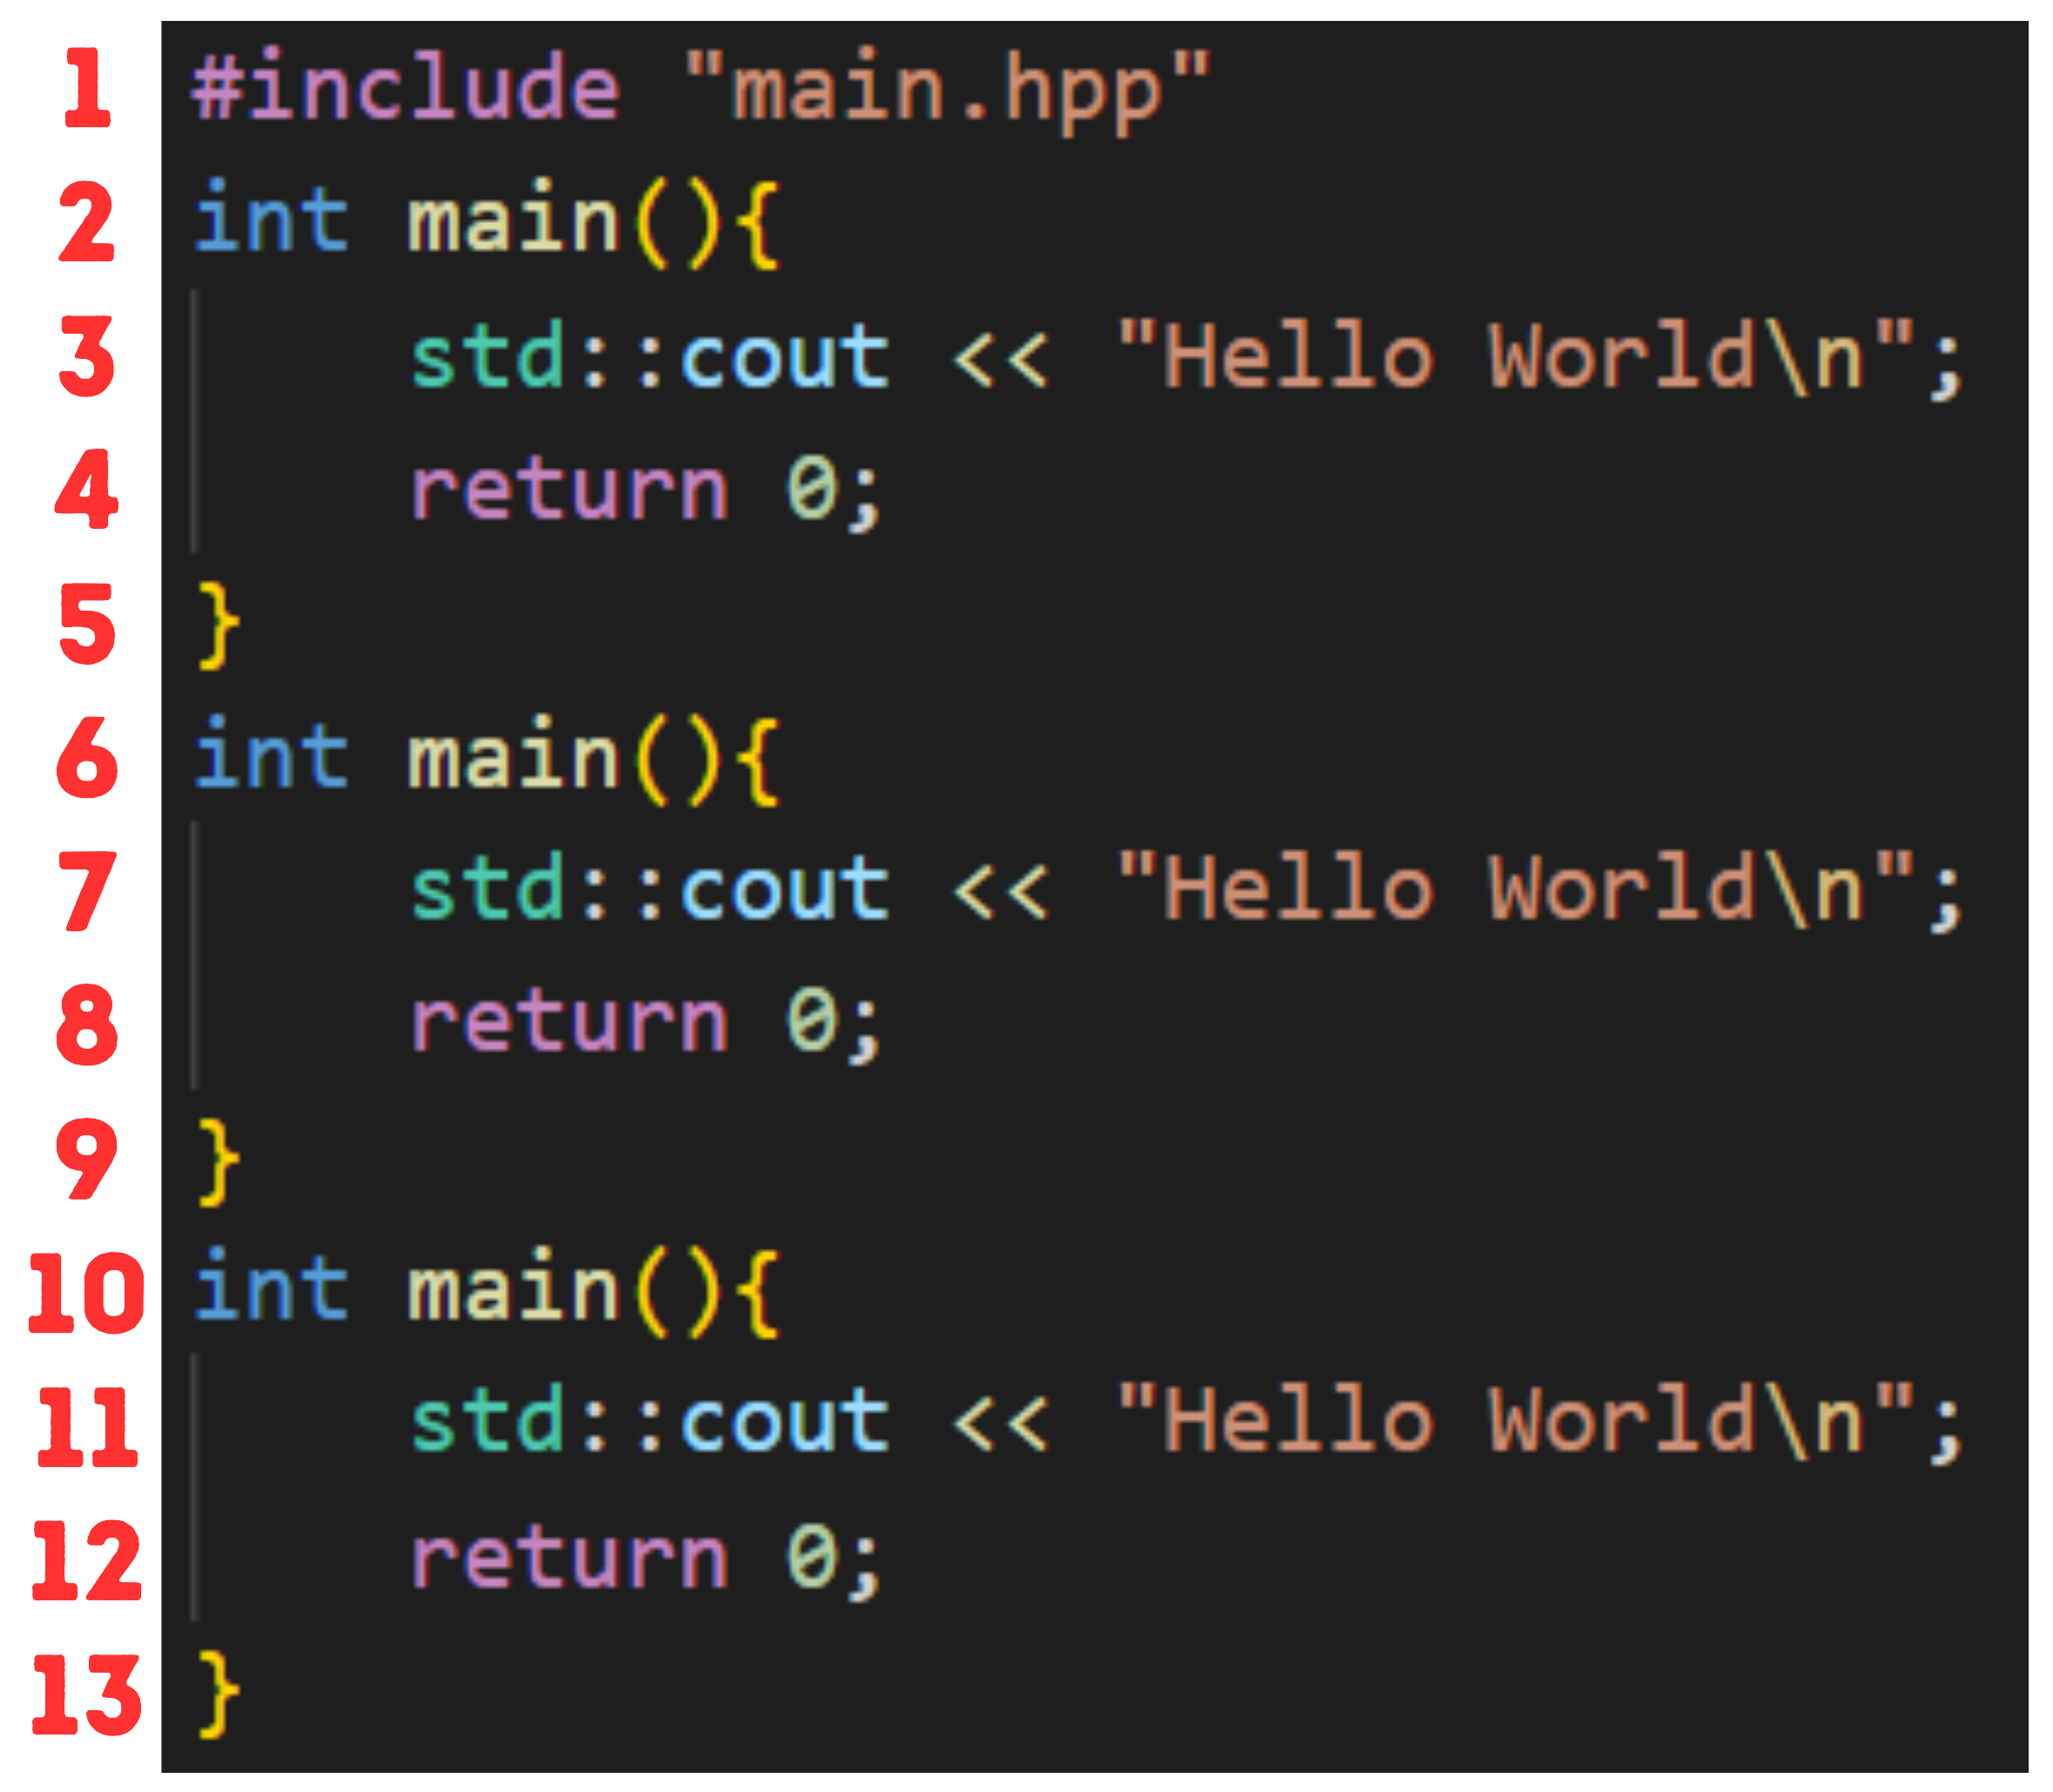
\includegraphics[width=0.3\textwidth]{include2.png}
  \caption{Illustration av den kompilerade filen i exempel 1. De röda siffrorna visar motsvarande radnummer
  i den kompilerade filen.}
  \label{fig:include1}
\end{figure}

\begin{figure}[h]
  \centering
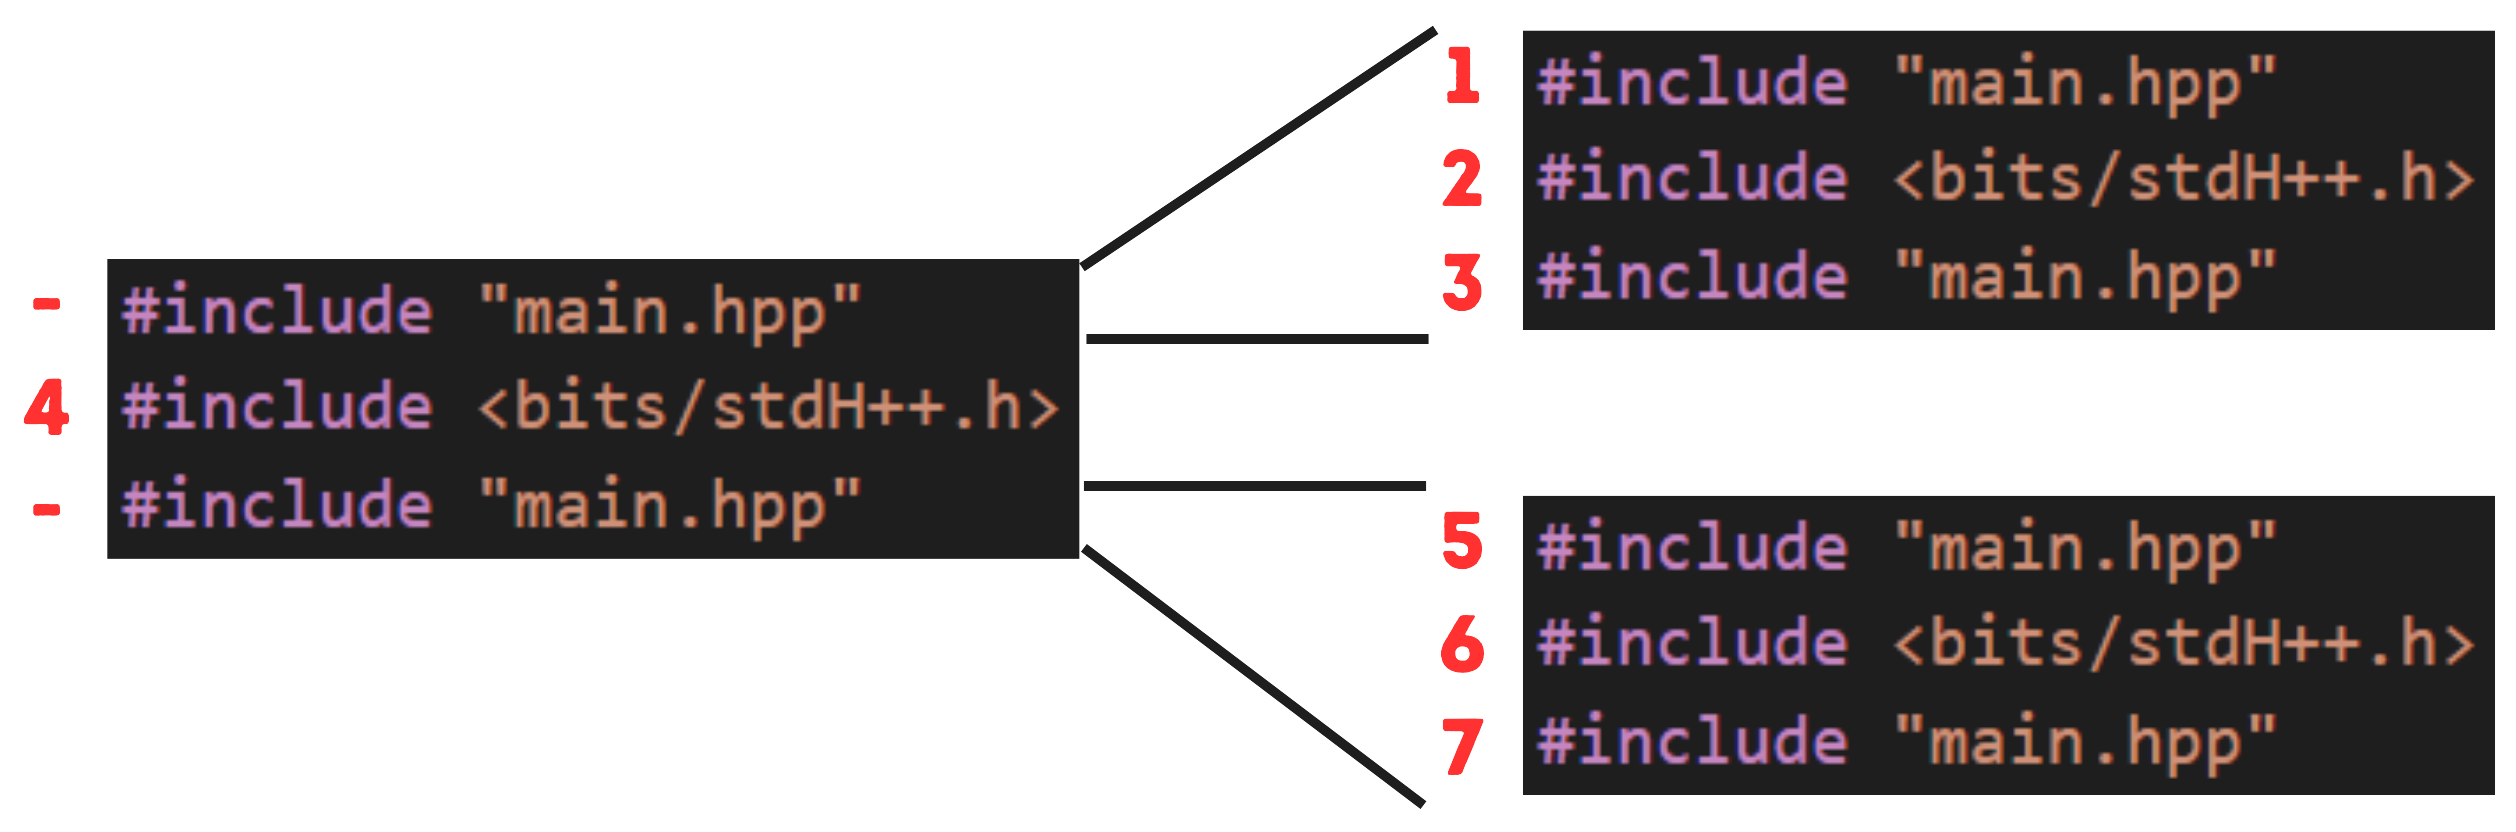
\includegraphics[width=0.8\textwidth]{include3.png}
  \caption{Illustration av exempel 3 med ursprungligen 3 rader. De röda siffrorna visar motsvarande radnummer
  i den kompilerade filen.}
  \label{fig:include1}
\end{figure}
